% Created 2020-11-10 Tue 15:10
% Intended LaTeX compiler: pdflatex
\documentclass[11pt]{article}
\usepackage[utf8]{inputenc}
\usepackage[T1]{fontenc}
\usepackage{graphicx}
\usepackage{grffile}
\usepackage{longtable}
\usepackage{wrapfig}
\usepackage{rotating}
\usepackage[normalem]{ulem}
\usepackage{amsmath}
\usepackage{textcomp}
\usepackage{amssymb}
\usepackage{capt-of}
\usepackage{hyperref}
\usepackage{minted}
\author{Ryan Greenup}
\date{\today}
\title{The Emergence of Patterns in Nature and Chaos Theory}
\hypersetup{
 pdfauthor={Ryan Greenup},
 pdftitle={The Emergence of Patterns in Nature and Chaos Theory},
 pdfkeywords={},
 pdfsubject={},
 pdfcreator={Emacs 27.1 (Org mode 9.4)}, 
 pdflang={English}}
\begin{document}

\maketitle
\tableofcontents

\section{Using Effort Estimates}
\label{sec:org94230b3}
The \href{https://orgmode.org/manual/Effort-Estimates.html}{Effort Estimages} in org-mode can be used to manage how much time each headline will take.

So first add the following to the header:

\begin{verbatim}
#+PROPERTY: Effort_ALL 0 0:10 0:30 1:00 2:00 3:00 4:00 5:00 6:00 7:00
#+COLUMNS: %40ITEM(Task) %17Effort(Estimated Effort){:} %CLOCKSUM
\end{verbatim}

Then add effort estimates to each headline by using \texttt{org-clock-modify-effort-estimate} which is bound to:

\begin{center}
\begin{tabular}{lll}
Emacs & C-C C-x C-e & \\
Doom & SPC m c e & \\
\end{tabular}

\end{center}

The effort Estimate should look something like this:

\begin{verbatim}
* My Fractal
:PROPERTIES:
:Effort:   0:02
:END:
\end{verbatim}


Then generate a a column view using  \texttt{M-x org-columns} which is bound to \texttt{C-c C-x C-c}, this will generate a layout that looks something like this:

\begin{center}
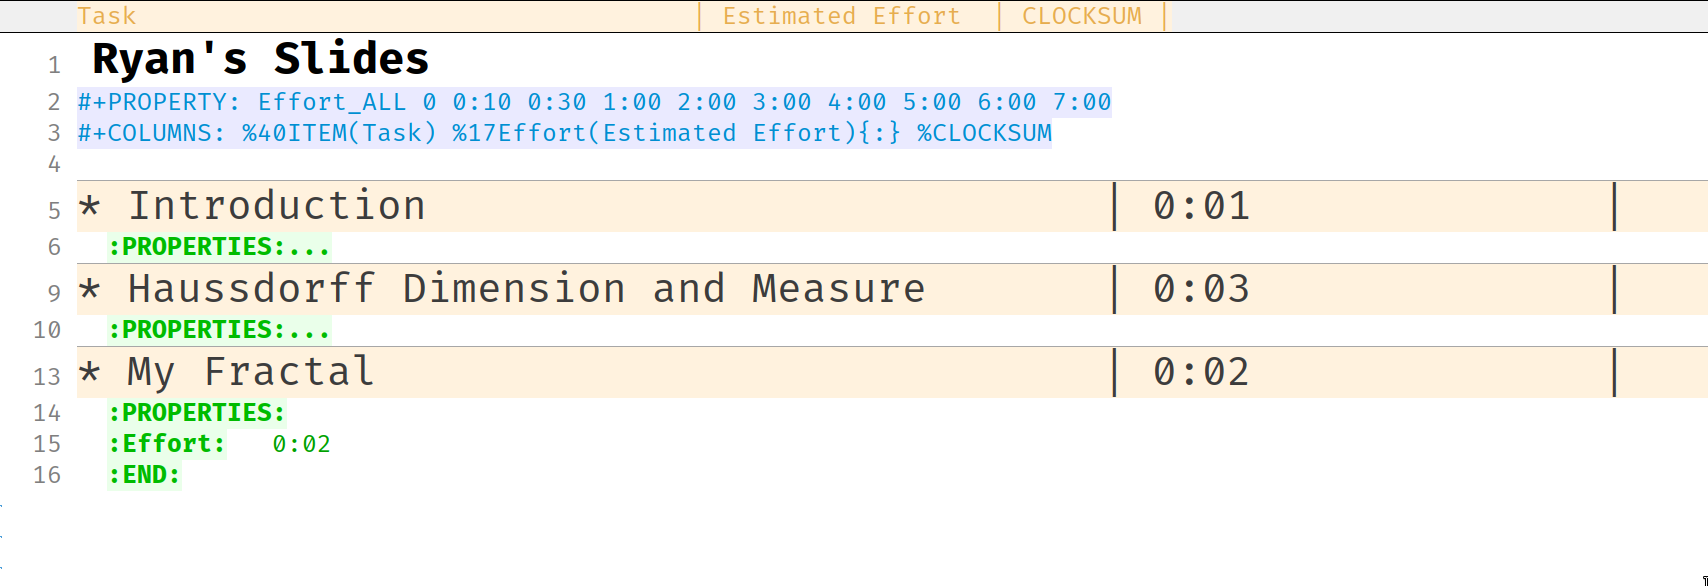
\includegraphics[width=0.4\textwidth]{media/screenshot-of-org-mode-column-view.png}
\end{center}

as text:

\begin{verbatim}
#+TITLE: Ryan's Slides
#+PROPERTY: Effort_ALL 0 0:10 0:30 1:00 2:00 3:00 4:00 5:00 6:00 7:00
#+COLUMNS: %40ITEM(Task) %17Effort(Estimated Effort){:} %CLOCKSUM

* Introduction
:PROPERTIES:
:Effort:   0:01
:END:
* Haussdorff Dimension and Measure
:PROPERTIES:
:Effort:   0:03
:END:
* My Fractal
:PROPERTIES:
:Effort:   0:02
:END:
\end{verbatim}
\end{document}
